\documentclass[handout,12pt]{beamer}

\hypersetup{colorlinks=true,linkcolor=red}
\usetheme{boxes}

\usepackage[utf8]{inputenc}
\usepackage[russian,english]{babel}
\usepackage[T2A]{fontenc}
\usepackage{hyperref}
\usepackage[final]{listings}
\usepackage{breakurl}
\usepackage{cite}
\usepackage{perpage}

\graphicspath{{img/}}

\def\Url\Breaks{\do\/\do-}
\lstset{
  frame=none,
  breaklines=true,
  basicstyle=\lst@ifdisplaystyle\tiny\fi,
  postbreak=\raisebox{0ex}{\ensuremath{\hookrightarrow\space}},
  numbers=left,
  showlines=true
}

\MakePerPage{footnote}

\title{Операционные Системы}
\subtitle{Синхронизация потоков}
\date{\today}

\begin{document}

  \begin{frame}
    \titlepage
  \end{frame}
  \begin{frame}[fragile]
\frametitle{Пример}
    \begin{columns}
        \begin{column}{.4\textwidth}
            \begin{lstlisting}
    .data
counter:
    .int 0

    .text
add_one:
    movq counter, %rax
    inc %rax
    movq rax, counter
    retq
            \end{lstlisting}
        \end{column}
        \begin{column}{.4\textwidth}
            \begin{lstlisting}
int counter;

int add_one(void)
{
    return ++counter;
}	
            \end{lstlisting}
        \end{column}
        \begin{column}{.2\textwidth}
        \end{column}
    \end{columns}
\end{frame}

\begin{frame}[fragile]
\frametitle{Вариант 1}
\begin{columns}
    \begin{column}{.35\textwidth}
        \begin{lstlisting}
movq counter, %rax
inc %rax
movq rax, counter
 
 
 
        \end{lstlisting}
    \end{column}
    \begin{column}{.35\textwidth}
        \begin{lstlisting}
 
 
 
movq counter, %rax
inc %rax
movq rax, counter
        \end{lstlisting}
    \end{column}
    \begin{column}{.3\textwidth}
    \end{column}
\end{columns}
\end{frame}

\begin{frame}[fragile]
\frametitle{Вариант 2}
\begin{columns}
    \begin{column}{.35\textwidth}
        \begin{lstlisting}
movq counter, %rax

inc %rax
movq rax, counter
 
 
        \end{lstlisting}
    \end{column}
    \begin{column}{.35\textwidth}
        \begin{lstlisting}
 
movq counter, %rax
 
 
inc %rax
movq rax, counter
        \end{lstlisting}
    \end{column}
    \begin{column}{.3\textwidth}
    \end{column}
\end{columns}
\end{frame}

\begin{frame}
\frametitle{Состояние гонки}
\begin{itemize}
    \item<1->Состояние гонки - результат зависит от порядка выполнения
         инструкций
    \begin{itemize}
        \item<2->порядок зависит от слишком многих факторов;
        \item<3->решения планировщика, влияние других потоков, прерывания...
        \item<4->могут быть трудно воспроизводимы - не поддаются тестированию.
    \end{itemize}
\end{itemize}
\end{frame}

\begin{frame}
\frametitle{Критическая секция}
\begin{itemize}
    \item<1->Критическая секция
    \begin{itemize}
        \item<2->участок кода, обращающийся к разделяемым несколькими потоками
             данным;
        \item<3->если не более, чем один поток может одновременно находиться в
             критической секции, то не будет состояния гонки.
    \end{itemize}
\end{itemize}
\end{frame}

\begin{frame}
\frametitle{Блокировка}
\begin{itemize}
    \item<1->Блокировка (lock) - некоторый объект и пара методов для работы с
         ним
    \begin{itemize}
        \item<2->lock - метод захвата блокировки;
        \item<3->unlock - метод освобождения блокировки.
    \end{itemize}
\end{itemize}
\end{frame}

\begin{frame}
\frametitle{Свойство взаимного исключения}
\begin{itemize}
    \item<1->Взaимное исключение (mutual exclusion)
    \begin{itemize}
        \item<2->потоки всегда вызывают lock и unlock парами (сначала lock,
             а потом unlock);
        \item<3->не более одного потока может одновременно находиться между
             lock-ом и unlock-ом.
    \end{itemize}
\end{itemize}
\end{frame}

\begin{frame}[fragile]
\frametitle{Свойство взаимного исключения}
\begin{lstlisting}
    struct lock l;
    int counter;

    int add_one(void)
    {
        int res;

        lock(&l);
        res = ++counter;
        unlock(&l);
    }
\end{lstlisting}
\end{frame}

\begin{frame}[fragile]
\frametitle{Свойство взаимного исключения}
\begin{columns}
    \begin{column}{.4\textwidth}
        \begin{lstlisting}
struct lock lock0;
int counter0;

int add_one0(void)
{
    int res;

    lock(&lock0);
    res = ++counter0;
    unlock(&lock0);
    return res;
}
        \end{lstlisting}
    \end{column}
    \begin{column}{.4\textwidth}
        \begin{lstlisting}
struct lock lock1;
int counter1;

int add_one1(void)
{
    int res;

    lock(&lock1);
    res = ++counter1;
    unlock(&lock1);
    return res;
}
        \end{lstlisting}
    \end{column}
    \begin{column}{.2\textwidth}
    \end{column}
\end{columns}
\end{frame}

\begin{frame}[fragile]
\frametitle{Свойство живости}
\begin{lstlisting}
    struct lock {
    };

    void lock(struct lock *unused)
    {
        (void) unused;
        while (1);
    }

    void unlock(struct lock *unused)
    {
        (void) unused;
    }
\end{lstlisting}
\end{frame}

\begin{frame}
\frametitle{Свойство живости}
\begin{itemize}
    \item<1->Свойство живости (deadlock freedom)
    \begin{itemize}
        \item<2->если один из потоков вызвал lock, то какой-то из
             потоков, вызвавших lock, захватит блокировку;
        \item<3->поток не ждет в lock, если он единственный пытается захватить
             блокировку;
        \item<4->если поток ждет, значит другому потоку повезло захватить
             блокировку.
    \end{itemize}
\end{itemize}
\end{frame}

\begin{frame}
\frametitle{На что нельзя полагаться?}
\begin{itemize}
    \item<1->Скорость работы потоков:
    \begin{itemize}
        \item<2->мы не знаем, сколько времени потребуется потоку, чтобы
             выполнить какой-то код;
        \item<3->мы не можем полагать, что какой-то поток быстрее.
    \end{itemize}
\end{itemize}
\end{frame}

\begin{frame}
\frametitle{На что можно полагаться?}
\begin{itemize}
    \item<1->Потоки работают корректно:
    \begin{itemize}
        \item<2->поток не находится между lock и unlock бесконечно;
        \item<3->поток не "падает", находясь между lock и unlock;
        \item<4->и так далее...
    \end{itemize}
\end{itemize}
\end{frame}

  \begin{frame}
\frametitle{Атомарный Read/Write регистр}
\begin{itemize}
    \item<1->Атомарный RW регистр - ячейка памяти и пара операций
    \begin{itemize}
        \item<2->write - "атомарно" записывает значение в регистр;
        \item<3->read - "атомарно" читает последнее записанное значение;
        \item<4->все операции (read/write) упорядочены.
    \end{itemize}
\end{itemize}
\end{frame}

\begin{frame}
\frametitle{Взаимное исключение для 2-х потоков}
\begin{itemize}
    \item<1->Есть всего два потока
    \begin{itemize}
        \item<2->потоки имеют идентификаторы 0 и 1;
        \item<3->внутри потока мы можем узнать его идентификатор (пусть за
             это отвечает функция \lstinline|threadId|).
    \end{itemize}
\end{itemize}
\end{frame}

\begin{frame}[fragile]
\frametitle{Альтернация}
\begin{lstlisting}
    struct lock {
        atomic_int last;
    };

    void lock_init(struct lock *lock)
    {
        atomic_store(&lock->last, 0);
    }

    void lock(struct lock *lock)
    {
        while (atomic_load(&lock->last) == threadId());
    }

    void unlock(struct lock *lock)
    {
        atomic_store(&lock->last, threadId());
    }
\end{lstlisting}
\end{frame}

\begin{frame}
\frametitle{Свойство взаимного исключения}
\begin{itemize}
    \item<1->Для приведенного алгоритма взаимное исключение гарантируется
    \begin{itemize}
        \item<2->lock может вернуть управление только потоку с
             идентификатором, не равным \lstinline|lock->last|;
        \item<3->только поток с \lstinline|threadId() != lock->last| может
             изменить значение \lstinline|lock->last|.
    \end{itemize}
\end{itemize}
\end{frame}

\begin{frame}
\frametitle{Свойство живости}
\begin{itemize}
    \item<1->Пусть поток 1 вообще никогда не пытается захватить лок
    \begin{itemize}
        \item<2->если поток 0 вызовет lock, то он зависнет навсегда;
        \item<3->т. е. свойство живости не выполняется.
    \end{itemize}
\end{itemize}
\end{frame}

\begin{frame}[fragile]
\frametitle{Флаги намерения}
\begin{lstlisting}
    struct lock {
        atomic_int flag[2];
    };

    void lock_init(struct lock *lock)
    {
        atomic_store(&lock->flag[0], 0);
        atomic_store(&lock->flag[1], 0);
    }

    void lock(struct lock *lock)
    {
        const int me = threadId();
        const int other = 1 - me;

        atomic_store(&lock->flag[me], 1);
        while (atomic_load(&lock->flag[other]));
    }

    void unlock(struct lock *lock)
    {
        const int me = threadId();

        atomic_store(&lock->flag[me], 0);
    }
\end{lstlisting}
\end{frame}

\begin{frame}
\frametitle{Корректность}
\begin{itemize}
    \item<1->Гарантируется ли взаимное исключение?
    \item<2->Гарантируется ли живость?
\end{itemize}
\end{frame}

\begin{frame}[fragile]
\frametitle{Алгоритм Петерсона для 2-х потоков}
\begin{lstlisting}
    struct lock {
        atomic_int last;
        atomic_int flag[2];
    };

    void lock(struct lock *lock)
    {
        const int me = threadId();
        const int other = 1 - me;

        atomic_store(&lock->flag[me], 1);
        atomic_store(&lock->last, me);

        while (atomic_load(lock->flag[other])
               && atomic_load(&lock->last) == me);
    }

    void unlock(struct lock *lock)
    {
        const int me = threadId();

        atomic_store(&lock->flag[me], 0);
    }
\end{lstlisting}
\end{frame}

\begin{frame}
\frametitle{Взаимное исключение}
\begin{itemize}
    \item<1->Доказательство от противного - пусть два потока одновременно
         находятся в критической секции
    \begin{itemize}
        \item<2->оба потока записывали значение в атомарный регистр last;
        \item<3->один из них должен был быть первым, а другой последним;
        \item<4->для определенности пусть последним был поток 1.
    \end{itemize}
\end{itemize}
\end{frame}

\begin{frame}
\frametitle{Взаимное исключение}
\begin{itemize}
    \item<1->Итак нам известно следующее:
    \begin{itemize}
        \item<2->\lstinline|lock->last == 1| - последним туда записал поток 1;
        \item<3->\lstinline|lock->flag[0] = 1| и \lstinline|lock->flag[1] == 1|.
    \end{itemize}
\end{itemize}
\end{frame}

\begin{frame}
\frametitle{Взаимное исключение}
\begin{itemize}
    \item<1->Как в таких условиях поток 1 мог пройти мимо цикла в lock и войти
         в критическую секцию?
    \begin{itemize}
        \item<2->очевидно, никак.
    \end{itemize}
\end{itemize}
\end{frame}

\begin{frame}
\frametitle{Живость}
\begin{itemize}
     \item<1->Пусть поток 0 пытается войти в критическую секцию, возможны две
          ситуации:
     \begin{itemize}
         \item<2->при проверке условия цикла \lstinline|lock->flag[1] == 0|;
         \item<3->при проверке условия цикла \lstinline|lock->flag[1] == 1|.
     \end{itemize}
\end{itemize}
\end{frame}

\begin{frame}
\frametitle{Живость}
\begin{itemize}
    \item<1->В первом случае (\lstinline|lock->flag[1] == 0|)
    \begin{itemize}
        \item<2->поток 1 даже не пытался захватить блокировку;
        \item<3->условие цикла, очевидно, ложно, и поток 0 входит в
             критическую секцию
    \end{itemize}
\end{itemize}
\end{frame}

\begin{frame}
\frametitle{Живость}
\begin{itemize}
    \item<1->Во втором случае (\lstinline|lock->flag[1] == 1|)
    \begin{itemize}
        \item<2->оба потока изъявили намерение войти в критическую секцию;
        \item<3->нужно показать, что хотя бы один из них рано или поздно
             войдет в критическую секцию (или уже там).
    \end{itemize}
\end{itemize}
\end{frame}

\begin{frame}
\frametitle{Живость}
\begin{itemize}
    \item<1->Оба потока после записи в \lstinline|lock->flag[x]| должны в
         какой-то момент записать в \lstinline|lock->last|
    \begin{itemize}
        \item<2->не трудно увидеть, что если \lstinline|lock->flag[0] == 1| и
             \lstinline|lock->flag[1] == 1|,
        \item<2->то тот из них, кто сделал это первым, войдет в критическую
             секцию.
    \end{itemize}
\end{itemize}
\end{frame}


\begin{frame}
\frametitle{N потоков}
\begin{itemize}
    \item<1->Реализовав взаимное исключение для 2-х потоков, мы можем
         реализовать вазимное исключение для любого числа потоков
    \begin{itemize}
        \item<2->организуем турнир для N потоков;
        \item<3->потоки конкурируют друг с другом на "выбывание".
    \end{itemize}
\end{itemize}
\end{frame}

\begin{frame}
\frametitle{N потоков}
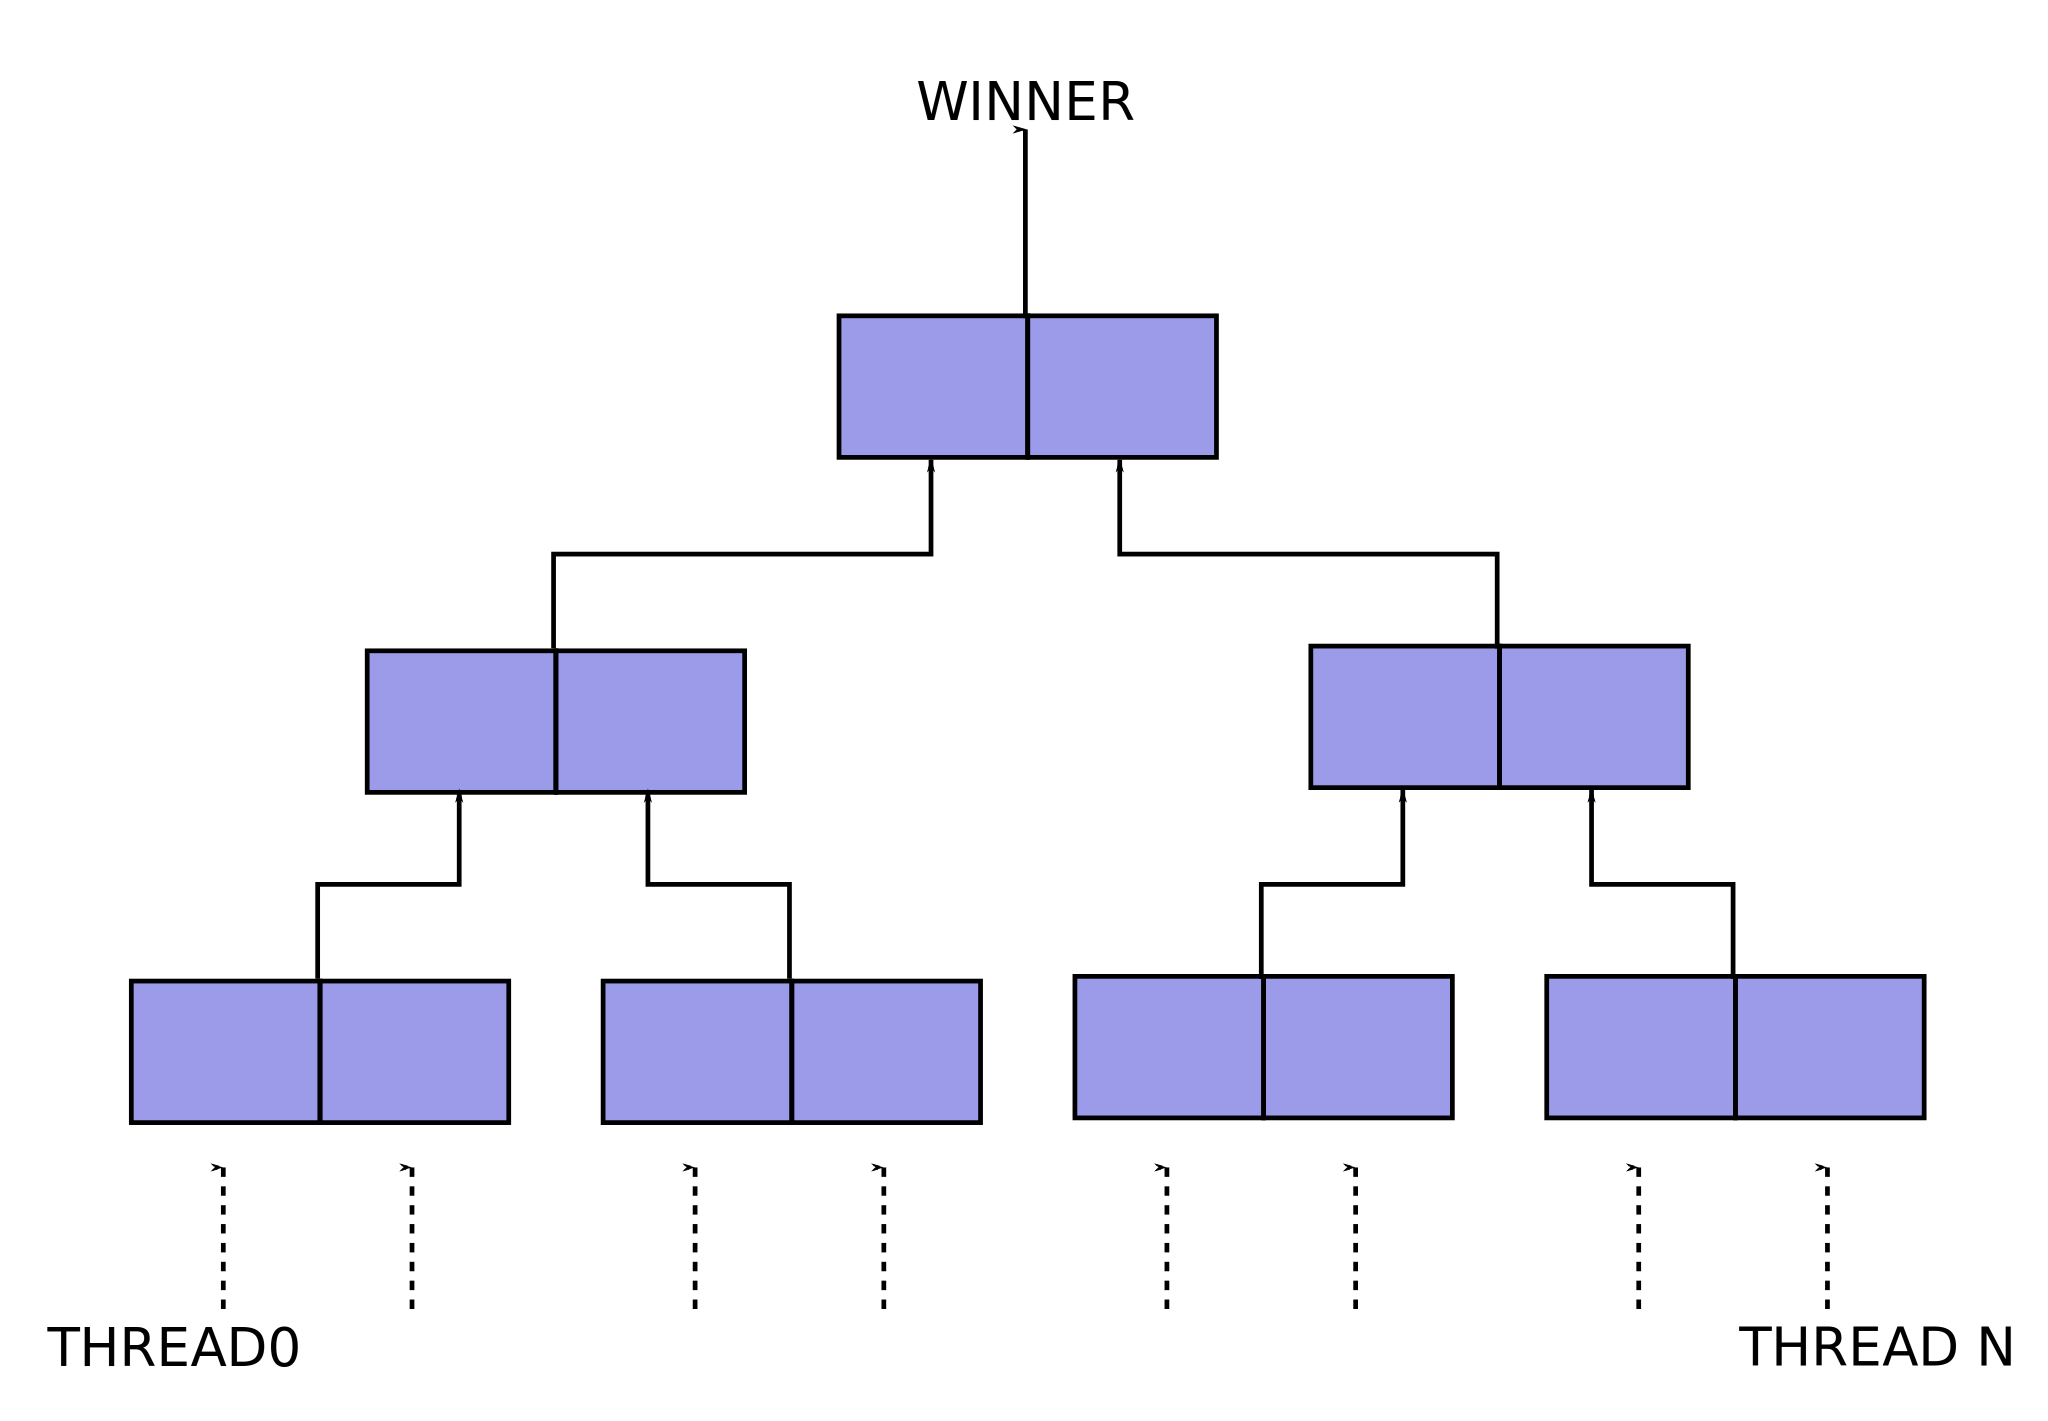
\includegraphics[height=.5\textheight]{nthreads}
\end{frame}

\begin{frame}[fragile]
\frametitle{Алгоритм Петерсона для N потоков}
\begin{lstlisting}
    struct lock_one {
        atomic_int last;
        atomic_int flag[N];
    };

    int flags_clear(const struct lock_one *lock)
    {
        const int me = threadId();

        for (int i = 0; i != N; ++i) {
            if (i != me && atomic_load(&lock->flag[i]))
                return 0;
        }
        return 1;
    }

    void lock_one(struct lock_one *lock)
    {
        const int me = threadId();

        atomic_store(&lock->flag[me], 1);
        atomic_store(&lock->last, me);

        while (!flags_clear(lock)
               && atomic_load(&lock->last) == me);
    }

    void unlock_one(struct lock_one *lock)
    {
        const int me = threadId();

        atomic_store(&lock->flag[me], 0);
    }
\end{lstlisting}
\end{frame}

\begin{frame}[fragile]
\frametitle{Алгоритм Петерсона для N потоков}
\begin{lstlisting}
    struct lock {
        struct lock_one lock[N - 1];
    };

    void lock(struct lock *lock)
    {
        for (int i = 0; i != N - 1; ++i)
            lock_one(&lock->lock[i]);
    }

    void unlock(struct lock *lock)
    {
        for (int i = N - 2; i >= 0; --i)
            unlock_one(&lock->lock[i]);
    }
\end{lstlisting}
\end{frame}

\begin{frame}[fragile]
\frametitle{Алгоритм Петерсона для N потоков}
\begin{lstlisting}
    struct lock {
        atomic_int level[N];
        atomic_int last[N - 1];
    };

    void lock(struct lock *lock)
    {
        const int me = threadId();

        for (int i = 0; i != N - 1; ++i) {
            atomic_store(&lock->level[me], i + 1);
            atomic_store(&lock->last[i], me);

            while (!flags_clear(lock, i)
                   && atomic_load(&lock->last[i]) == me);
        }
    }

    void unlock(struct lock *lock)
    {
        const int me = threadId();

        atomic_store(&lock->level[me], 0);
    }
\end{lstlisting}
\end{frame}

\begin{frame}
\frametitle{Честность}
\begin{itemize}
    \item<1->Не хочется, чтобы потоки голодали!
    \begin{itemize}
        \item<2->если поток захотел захватить блокировку, то когда-нибудь
             ему это удастся;
        \item<3->сравните с живостью - среди потоков, пытающихся захватить
             блокировку, одному это удастся.
    \end{itemize}
\end{itemize}
\end{frame}

\begin{frame}
\frametitle{Супер честность}
\begin{itemize}
    \item<1->k-ограниченное ожидание:
    \begin{itemize}
        \item<2->после того как поток "изъявил" желание захватить блокировку
             (встал в очередь), не более k потоков могут пролезть вперед него
             без очереди.
    \end{itemize}
\end{itemize}
\end{frame}

\begin{frame}
\frametitle{Алгоритм Петерсона на примере 3 потоков}
\begin{table}
\begin{tabular}{l | c | c | c | c | c }
№ & level[0] & level[1] & level[2] & last[0] & last[1] \\
\hline\hline

0 & 0 & 0 & 0 & 0 & 0 \\
1 & 1 & 0 & 0 & 0 & 0 \\
2 & 1 & 1 & 0 & 1 & 0 \\
3 & 1 & 1 & 1 & 2 & 0 \\
4 & 2 & 1 & 1 & 2 & 0 \\
5 & 0 & 1 & 1 & 2 & 0 \\
6 & 1 & 1 & 1 & 0 & 0 \\
7 & 1 & 1 & 2 & 0 & 2 \\
8 & 1 & 1 & 0 & 0 & 2 \\
9 & 1 & 1 & 1 & 2 & 2 \\
10 & 2 & 1 & 1 & 2 & 0 \\

\hline
\end{tabular}
\end{table}
\end{frame}

  \begin{frame}
\frametitle{Атомарный Read/Modify/Write регистр}
\begin{itemize}
    \item<1->Атомарный RMW регистр позволяет за одну операцию
    \begin{itemize}
        \item<2->прочитать значение в регистре;
        \item<3->преобразовать некоторым образом прочитанное значение;
        \item<4->записать преобразованное значение назад.
    \end{itemize}
\end{itemize}
\end{frame}

\begin{frame}[fragile]
\frametitle{Атомарный Read/Modify/Write регистр}
\begin{lstlisting}
    int atomic_rmw(int *reg, int (*f)(int))
    {
        const int old = *reg;
        const int new = f(old);

        *reg = new;
        return old;
    }
\end{lstlisting}
\end{frame}

\begin{frame}
\frametitle{Атомарный Read/Modify/Write регистр}
\begin{itemize}
    \item<1->\lstinline|atomic_exchange| - возвращает старое значение,
         записывает новое;
    \item<2->\lstinline;atomic_fetch_\{add|sub|or|and|xor\}; - выполняет
         арифметическое дествие над атомарным регистром;
    \item<3->\lstinline|atomic_compare_exchange| - записывает новое значение,
         если старое значение равно заданному.
\end{itemize}
\end{frame}

\begin{frame}
\frametitle{Реализация RMW регистра}
\begin{itemize}
    \item<1->Архитектура может поддерживать RMW операции (x86 - одна из них)
    \begin{itemize}
        \item<2->\lstinline|xchg|;
        \item<3->\lstinline|lock add|, \lstinline|lock sub|,
             \lstinline|lock or|, \lstinline|lock and|, \lstinline|lock xor|;
        \item<4->\lstinline|lock cmpxchg|.
    \end{itemize}
\end{itemize}
\end{frame}

\begin{frame}
\frametitle{Реализация RMW регистра}
\begin{itemize}
    \item<1->Архитектура может поддерживать LL/SC (например, ARM):
    \begin{itemize}
        \item<2->LL (load-link, load-linked, load-locked) - загружает значение
             из памяти;
        \item<3->SC (store-conditional) - записывает новое значение в ячейку,
             но только если после LL эту ячейку никто не трогал;
        \item<4->LL/SC идут парами и работают вместе как одна RMW операция.
    \end{itemize}
\end{itemize}
\end{frame}

\begin{frame}[fragile]
\frametitle{Взаимное исключение с использованием RWM регистра}
\begin{lstlisting}
    #define LOCKED   1
    #define UNLOCKED 0

    struct lock {
        atomic_int locked;
    };

    void lock(struct lock *lock)
    {
        while (atomic_exchange(&lock->locked, LOCKED) != UNLOCKED);
    }

    void unlock(struct lock *lock)
    {
        atomic_store(&lock->locked, UNLOCKED);
    }
\end{lstlisting}
\end{frame}

\begin{frame}
\frametitle{И снова про честность}
\begin{itemize}
    \item<1->Что если блокировка находится под нагрузкой (high contention)?
    \begin{itemize}
        \item<2->т. е. блокировка практически всегда занята;
        \item<3->некоторый поток может получать CPU только тогда, когда
             блокировка занята;
        \item<4->такой поток будет голодать - блокировка не честная.
    \end{itemize}
\end{itemize}
\end{frame}

\begin{frame}[fragile]
\frametitle{Ticket lock}
\begin{lstlisting}
    struct lock {
        atomic_uint ticket;
        atomic_uint next;
    };

    void lock(struct lock *lock)
    {
        const unsigned ticket = atomic_fetch_add(&lock->ticket, 1);

        while (atomic_load(&lock->next) != ticket);
    }

    void unlock(struct lock *lock)
    {
        atomic_fetch_add(&lock->next, 1);
    }
\end{lstlisting}
\end{frame}

\begin{frame}
\frametitle{И снова о прерываниях}
\begin{itemize}
    \item<1->Пусть у нас есть устройство, которое получает данные из сети
    \begin{itemize}
        \item<2->устройство сигналит процессору - генерирует прерывание;
        \item<3->процессор вызывает обработчик прерывания - функцию ядра ОС;
        \item<4->обработчик прерывания должен забрать данные с устройства и
             положить их в буфер, из которого какой-то поток сможет их забрaть.
    \end{itemize}
\end{itemize}
\end{frame}

\begin{frame}
\frametitle{И снова о прерываниях}
\begin{itemize}
    \item<1->Что если к этому буферу могут обращаться из нескольких потоков?
    \begin{itemize}
        \item<2->мы должны защитить буфер блокировкой;
        \item<3->потоки и обработчики прерываний должны захватывать эту
             блокировку перед обращением к буферу;
        \item<4->что если обработчик прерывания устройства прервал поток,
             который захватил блокировку?
    \end{itemize}
\end{itemize}
\end{frame}

\begin{frame}
\frametitle{Deadlock}
\begin{itemize}
    \item<1->Прерванный поток и обработчик прерывания ждут друг друга:
    \begin{itemize}
        \item<2->обработчик прерывания не может захватить блокировку, потому
             что ее держит прерванный поток;
        \item<3->пока обработчик прерывания не завершится, прерванный поток не
             получит управление и не сможет отпустить блокировку.
    \end{itemize}
\end{itemize}
\end{frame}

\begin{frame}
\frametitle{Мораль}
\begin{itemize}
    \item<1->Если блокировка защищает данные, к которым обращается обработчик
         прерывания, то нужно выключать прерывания
    \begin{itemize}
        \item<2->если прерывания отключены, то deadlock между обработчиком
             прерывания и прерванным потоком не может возникнуть.
    \end{itemize}
\end{itemize}
\end{frame}

\begin{frame}
\frametitle{Однопроцессорные системы}
\begin{itemize}
    \item<1->Представим систему с всего одним ядром/процессором
    \begin{itemize}
        \item<2->запретив прерывания и переключение потоков, мы получаем CPU в
             монопольное пользование;
        \item<3->все рассмотренные ранее алгоритмы просто не нужны.
    \end{itemize}
\end{itemize}
\end{frame}

  \begin{frame}
\frametitle{Разделение на читателей и писателей}
\begin{itemize}
    \item<1->Не все запросы к разделяемым данным одинаковы
    \begin{itemize}
        \item<2->есть запросы, которые модифицируют данные;
        \item<3->есть запросы, которые только читают данные.
    \end{itemize}
\end{itemize}
\end{frame}

\begin{frame}[fragile]
\frametitle{Разделение на читателей и писателей}
\begin{lstlisting}
    struct rwlock {
        atomic_uint ticket;
        atomic_uint write;
        atomic_uint read;
    };

    void read_lock(struct rwlock *lock)
    {
        const unsigned ticket = atomic_fetch_add(&lock->ticket, 1);

        while (atomic_load(&lock->read) != ticket);
        atomic_store(&lock->read, ticket + 1);
    }

    void read_unlock(struct rwlock *lock)
    {
        atomic_fetch_add(&lock->write, 1);
    }
\end{lstlisting}
\end{frame}

\begin{frame}[fragile]
\frametitle{Разделение на читателей и писателей}
\begin{lstlisting}
    struct rwlock {
        atomic_uint ticket;
        atomic_uint write;
        atomic_uint read;
    };

    void write_lock(struct rwlock *lock)
    {
        const unsigned ticket = atomic_fetch_add(&lock->ticket, 1);

        while (atomic_load(&lock->write) != ticket);
    }

    void write_unlock(struct rwlock *lock)
    {
        atomic_fetch_add(&lock->read, 1);
        atomic_fetch_add(&lock->write, 1);
    }
\end{lstlisting}
\end{frame}

  \begin{frame}
\frametitle{Стратегии ожидания}
\begin{itemize}
    \item<1->До сих пор функция lock всегда просто ждала в цикле
    \begin{itemize}
        \item<2->такая стратегия называется активным ожиданием;
        \item<3->блокировки, использующие активное ожидание, часто называются
             spinlock-ами;
        \item<3->они "крутятся" в цикле.
    \end{itemize}
\end{itemize}
\end{frame}

\begin{frame}
\frametitle{Активное ожидание}
\begin{itemize}
    \item<1->Активное ожидание хорошо работает если:
    \begin{itemize}
        \item<2->потоки не держат блокировку очень долго;
        \item<3->блокировка не находится под сильной нагрузкой;
        \item<4->т. е. если активное ожидание длится недолго.
    \end{itemize}
\end{itemize}
\end{frame}

\begin{frame}
\frametitle{Альтернативы активному ожиданию}
\begin{itemize}
    \item<1->Как можно ожидать не активно?
    \begin{itemize}
        \item<2->можно добровольно отдать CPU (переключиться на другой поток);
        \item<3->можно пометить поток как неактивный, чтобы планировщик не
             давал ему время на CPU, пока блокировка не будет отпущена.
    \end{itemize}
\end{itemize}
\end{frame}

  \begin{frame}
\frametitle{Задача Producer-а и Consumer-а}
\begin{itemize}
    \item<1->Рассмотрим следующую задачу:
    \begin{itemize}
        \item<2->Producer - поток/потоки, который генерирует данные;
        \item<3->Consumer - поток/потоки, который потребляет данные;
        \item<4->что если Producer и Consumer работают с разной скоростью?
    \end{itemize}
\end{itemize}
\end{frame}

\begin{frame}
\frametitle{Переменная состояния}
\begin{itemize}
    \item<1->Перемeнная состояния (condition variable) - объект и несколько
         методов для работы с ним
    \begin{itemize}
        \item<2->wait - ожидает, пока кто-нибудь не просигналит;
        \item<3->notify\_one - просигналить одному из ожидающих;
        \item<4->notify\_all - просигналить всем ожидающим.
    \end{itemize}
\end{itemize}
\end{frame}

\begin{frame}[fragile]
\frametitle{Переменная состояния}
\begin{lstlisting}
    struct lock;
    void lock(struct lock *lock);
    void unlock(struct lock *lock);

    struct condition;
    void wait(struct condition *cv, struct lock *lock);
    void notify_one(struct condition *cv);
    void notify_all(struct condition *cv);
\end{lstlisting}
\end{frame}

\begin{frame}[fragile]
\frametitle{Producer}
\begin{lstlisting}
    struct condition cv;
    struct lock mtx;
    int value;
    bool valid_value;
    bool done;

    void produce(int x)
    {
        lock(&mtx);
        while (valid_value)
            wait(&cv, &mtx);
        value = x;
        valid_value = true;
        notify_one(&cv);
        unlock(&mtx);
    }

    void finish(void)
    {
        lock(&mtx);
        done = true;
        notify_all(&cv);
        unlock(&mtx);
    }
\end{lstlisting}
\end{frame}

\begin{frame}[fragile]
\frametitle{Consumer}
\begin{lstlisting}
    int consume(int *x)
    {
        int ret = 0;
        lock(&mtx);

        while (!valid_value && !done)
            wait(&cv, &mtx);

        if (valid_value) {
            *x = value;
            valid_value = false;
            notify_one(&cv);
            ret = 1;
        }
        unlock(&mtx);
        return ret;
    }
\end{lstlisting}
\end{frame}

\begin{frame}[fragile]
\frametitle{Зачем нам lock?}
\begin{columns}
    \begin{column}{.4\textwidth}
        \begin{lstlisting}


/* lock(&mtx); */
done = true;
notify_all(&cv);
/* unlock(&mtx); */



        \end{lstlisting}
    \end{column}
    \begin{column}{.4\textwidth}
        \begin{lstlisting}
/* lock(&mtx); */
while (... && !done)




    wait(&cv, &mtx);
...
/* unlock(&mtx); */
        \end{lstlisting}
    \end{column}
    \begin{column}{.2\textwidth}
    \end{column}
\end{columns}
\end{frame}

\begin{frame}
\frametitle{Зачем нам цикл?}
\includegraphics[height=.6\textheight]{cv}
\end{frame}

\begin{frame}
\frametitle{Зачем нам цикл?}
\begin{itemize}
    \item<1->Spurious wakeups (ложные пробуждения) - ситуация, когда wait
         возвращает управление, даже если никто не сигналил
    \begin{itemize}
        \item<2->многие реализации переменной состояния подвержены:
        \begin{itemize}
            \item<3->С++;
            \item<4->Java;
            \item<5->POSIX Threads...
        \end{itemize}
    \end{itemize}
\end{itemize}
\end{frame}

  \begin{frame}
\frametitle{Deadlock}
\begin{itemize}
    \item<1->Deadlock - ситуация, при которой потоки не могут работать,
         потому что ждут друг друга:
    \begin{itemize}
        \item<2->deadlock потоком исполнения и обработчиком прерывания;
        \item<3->поток A ждет, пока поток B что-то сделает (например, отпустит
             блокировку);
        \item<4->а поток B ничего не делает, потому что ждет, пока поток A
             что-то сделает (например, отпустит блокировку).
    \end{itemize}
\end{itemize}
\end{frame}

\begin{frame}[fragile]
\frametitle{Пример}
\begin{columns}
    \begin{column}{.35\textwidth}
        \begin{lstlisting}
struct lock a;

void thread0(void)
{
    lock(&a);
    lock(&b);

    /* do something */

    unlock(&a);
    unlock(&b);
}
        \end{lstlisting}
    \end{column}
    \begin{column}{.35\textwidth}
        \begin{lstlisting}
struct lock b;

void thread1(void)
{
    lock(&b);
    lock(&a);

    /* do something else */

    unlock(&a);
    unlock(&b);
}
        \end{lstlisting}
    \end{column}
    \begin{column}{.3\textwidth}
    \end{column}
\end{columns}
\end{frame}

\begin{frame}[fragile]
\frametitle{Пример}
\begin{columns}
    \begin{column}{.35\textwidth}
        \begin{lstlisting}
    lock(&a);

    lock(&b);

        \end{lstlisting}
    \end{column}
    \begin{column}{.35\textwidth}
        \begin{lstlisting}

    lock(&b);

    lock(&a);
        \end{lstlisting}
    \end{column}
    \begin{column}{.3\textwidth}
    \end{column}
\end{columns}
\end{frame}

\begin{frame}
\frametitle{Wait-for граф}
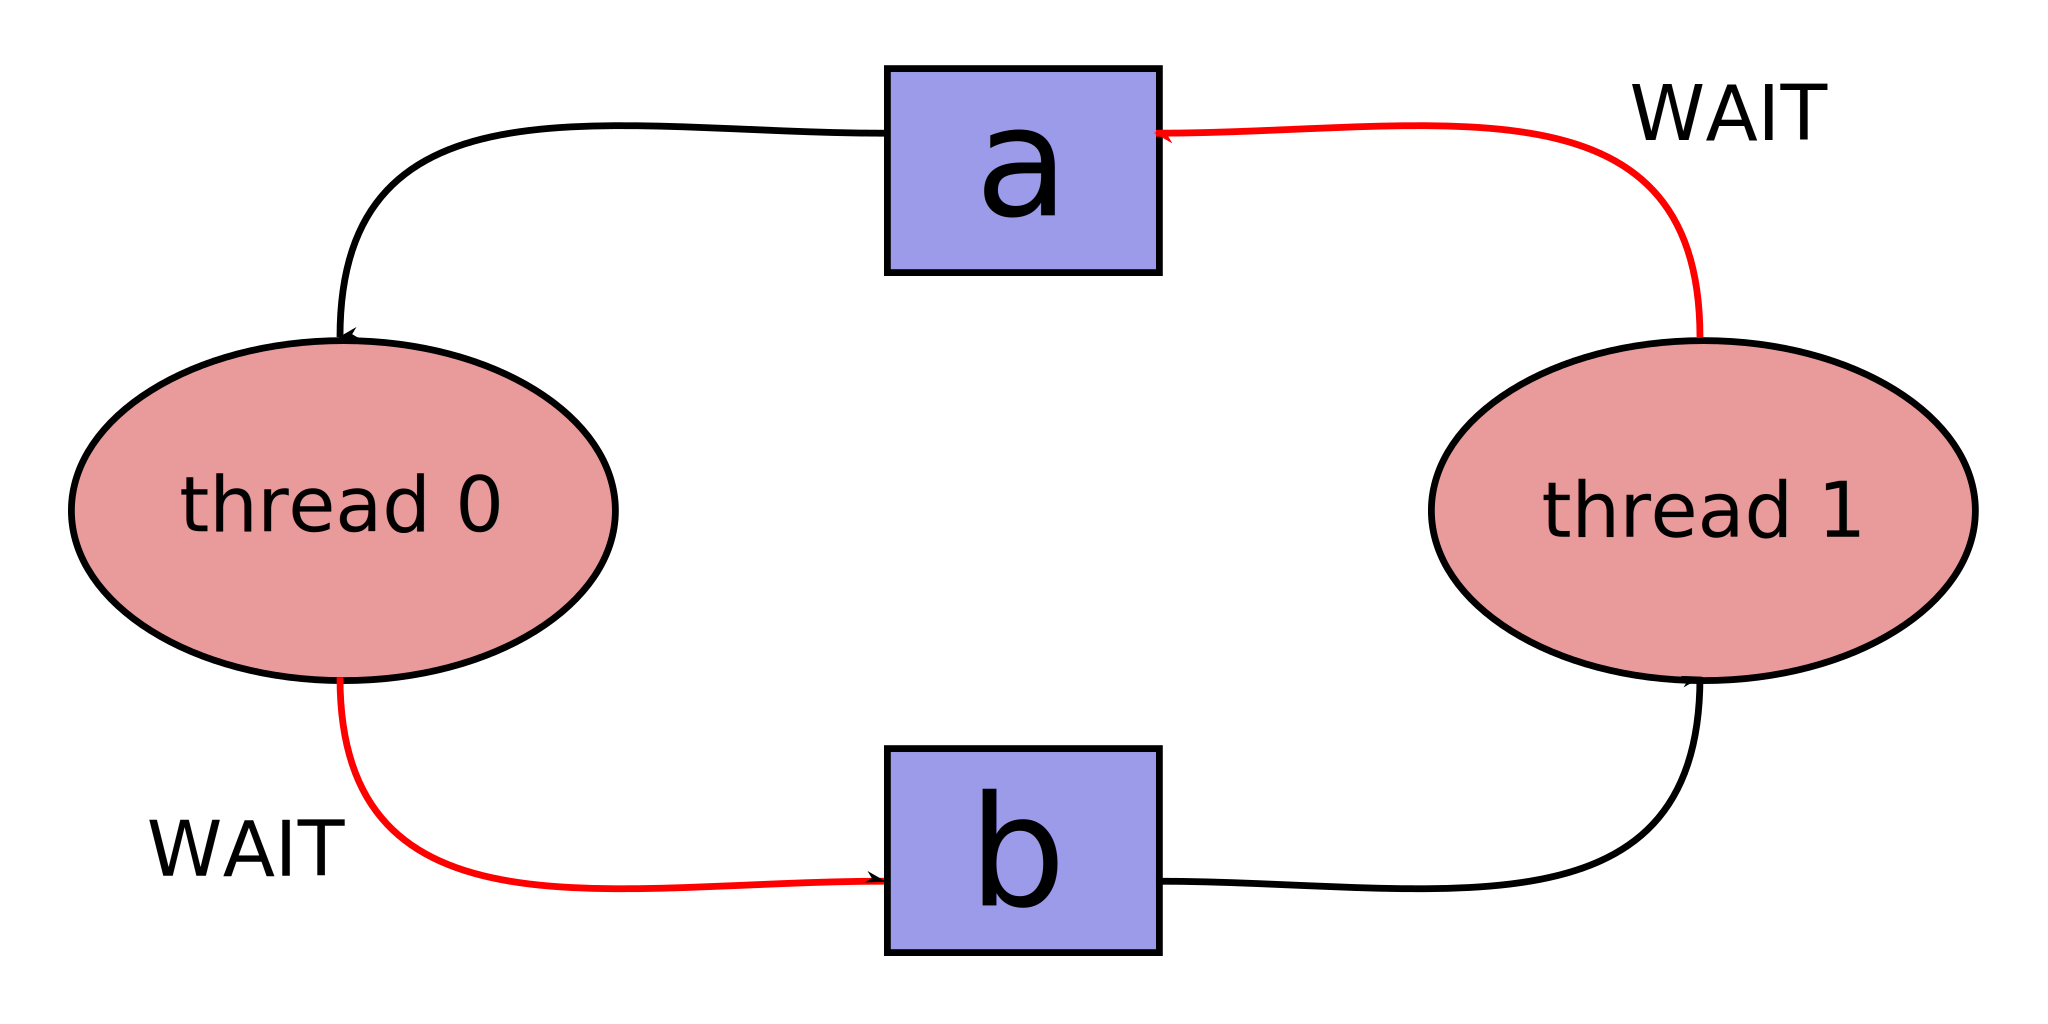
\includegraphics[height=.4\textheight]{waitfor}
\end{frame}

\begin{frame}
\frametitle{Deadlock}
\begin{itemize}
    \item<1->Как и с состоянием гонки, deadlock не поддается тестированию
    \begin{itemize}
        \item<2->появление зависит от многих факторов;
        \item<3->входные данные, решения планировщика, прерывания,
             производительность оборудования ...
    \end{itemize}
\end{itemize}
\end{frame}

\begin{frame}
\frametitle{Предотвращение deadlock-ов}
\begin{itemize}
    \item<1->Мы хотим избежать появления цикла в wait-for графе
    \begin{itemize}
        \item<2->простой случай - все блокировки известны заранее;
        \item<3->упорядочим все блокировки (например, по адресу);
        \item<4->захватываем блокировки только по порядку.
    \end{itemize}
\end{itemize}
\end{frame}

\begin{frame}[fragile]
\frametitle{Пример}
\begin{columns}
    \begin{column}{.35\linewidth}
        \begin{lstlisting}
void thread0()
{
    lock(&a);
    lock(&b);
    ...
    unlock(&b);
    unlock(&a);
}
        \end{lstlisting}
        \begin{lstlisting}
void thread2()
{
    lock(&c);
    lock(&a);
    ...
    unlock(&a);
    unlock(&c);
}
        \end{lstlisting}
    \end{column}
    \begin{column}{.35\linewidth}
        \begin{lstlisting}
void thread1()
{
    lock(&b);
    lock(&c);
    ...
    unlock(&c);
    unlock(&b);
}
        \end{lstlisting}
    \end{column}
    \begin{column}{.3\linewidth}
    \end{column}
\end{columns}
\end{frame}

\begin{frame}
\frametitle{Пример}
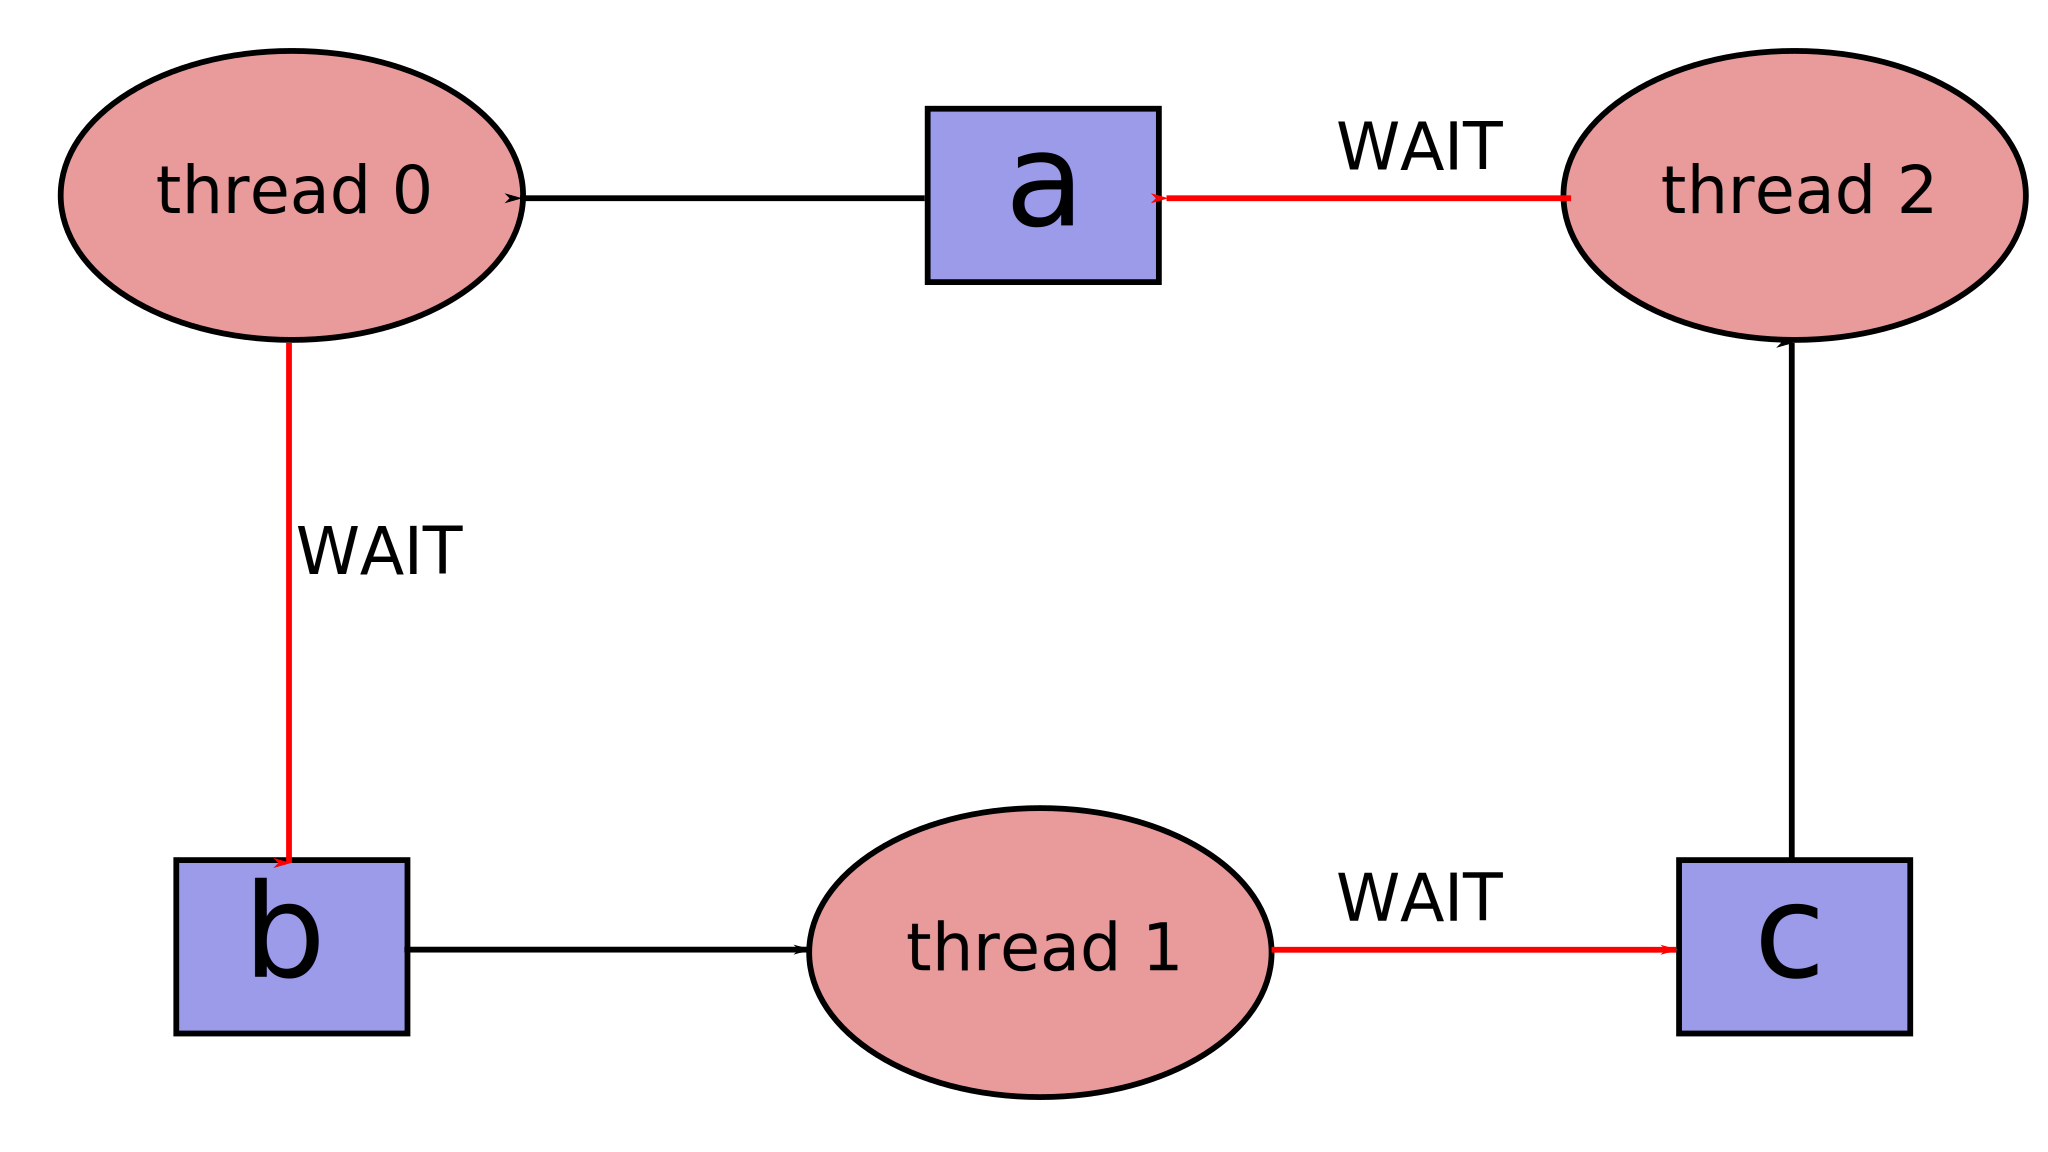
\includegraphics[height=.4\textheight]{order}
\end{frame}

\begin{frame}
\frametitle{Пример}
\begin{itemize}
    \item<1->Отсортируем блокировки a, b и c по алфавиту:
    \begin{itemize}
        \item<2->каждый поток должен захватывать блокировки только согласно
             порядку;
        \item<3->например, поток 2 хочет захватить блокировки c и a:
        \begin{itemize}
            \item<4->так как a в алфавтие раньше c, то сначала хватаем a,
            \item<5->потом хватаем c.
        \end{itemize}
    \end{itemize}
\end{itemize}
\end{frame}

\begin{frame}[fragile]
\frametitle{Пример}
\begin{columns}
    \begin{column}{.35\linewidth}
        \begin{lstlisting}
void thread0()
{
    lock(&a);
    lock(&b);
    ...
    unlock(&b);
    unlock(&a);
}
        \end{lstlisting}
        \begin{lstlisting}
void thread2()
{
    lock(&a);
    lock(&c);
    ...
    unlock(&c);
    unlock(&a);
}
        \end{lstlisting}
    \end{column}
    \begin{column}{.35\linewidth}
        \begin{lstlisting}
void thread1()
{
    lock(&b);
    lock(&c);
    ...
    unlock(&c);
    unlock(&b);
}
        \end{lstlisting}
    \end{column}
    \begin{column}{.3\linewidth}
    \end{column}
\end{columns}
\end{frame}

\begin{frame}
\frametitle{Предотвращение deadlock-ов}
\begin{itemize}
    \item<1->Сложный случай - все блокировки не известны заранее:
    \begin{itemize}
        \item<2->для этого случая придумано много различных вариантов;
        \item<3->мы рассмотрим подход, который называется Wait-Die.
    \end{itemize}
\end{itemize}
\end{frame}

\begin{frame}[fragile]
\frametitle{Изменим интерфейс}
\begin{lstlisting}
    struct wdlock_ctx {
        unsigned long long timestamp;
	struct wdlock *next;
    };

    struct wdlock {
        ...
    };

    /* Grab unique "timestamp" */
    void wdlock_ctx_init(struct wdlock_ctx *ctx);

    /* This function may fail */
    int wdlock_lock(struct wdlock *lock,
                    struct wdlock_ctx *ctx);

    /* Unlocks all of the locks */
    void wdlock_unlock(struct wdlock_ctx *ctx);
\end{lstlisting}
\end{frame}

\begin{frame}[fragile]
\frametitle{Как использовать Wait-Die подход?}
\begin{lstlisting}
    void thread(void)
    {
        struct wdlock_ctx ctx;

        wdlock_ctx_init(&ctx);

        while (1) {
            ...
            if (!wdlock_lock(&lock1, &ctx)) {
                wdlock_unlock(&ctx);
                continue;
            }
            ...
            if (!wdlock_lock(&lock2, &ctx)) {
                wdlock_unlock(&ctx);
                continue;
            }
            ...
        }
        /* Acquired all required locks successfully,
           can do something. */
        wdlock_unlock(&ctx);
    }
\end{lstlisting}
\end{frame}

\begin{frame}
\frametitle{"Контекст"}
\begin{itemize}
    \item<1->Wait-Die контекст состоит из:
    \begin{itemize}
        \item<2->списка захваченных блокировок;
        \item<3->уникального "timestamp".
    \end{itemize}
\end{itemize}
\end{frame}

\begin{frame}[fragile]
\frametitle{"Контекст"}
\begin{lstlisting}
    struct wdlock_ctx {
        unsigned long long timestamp;
	struct wdlock *next;
    };


    void wdlock_ctx_init(struct wdlock_ctx *ctx)
    {
        static atomic_ullong timestamp;

        ctx->timestamp = atomic_fetch_add(&timestamp, 1) + 1;
        ctx->next = NULL;
    }
\end{lstlisting}
\end{frame}

\begin{frame}
\frametitle{Магия timestamp}
\begin{itemize}
    \item<1->timestamp позволяет избегать deadlock-ов
    \begin{itemize}
        \item<2->храним в каждой блокировке timestamp из wdlock\_ctx, который
             использовали при захвате блокировки;
        \item<3->при попытке захватить блокировку возможно несколько вариантов:
        \begin{itemize}
            \item<4->если блокировка свободна, то пытаемся ее захватить - как
                 обычно;
            \item<5->если блокировка занята, то нужно сравнить timestamp-ы.
        \end{itemize}
    \end{itemize}
\end{itemize}
\end{frame}

\begin{frame}
\frametitle{Магия timestamp}
\begin{itemize}
    \item<1->Если блокировка захвачена, то нужно сравнить наш timestamp с
         сохраненным в блокировке:
    \begin{itemize}
        \item<2->если наш timestamp меньше, чем timestamp блокировки, то ждем;
        \item<3->в противном случае не ждем, а возвращаем признак неудачи
             (умираем).
    \end{itemize}
\end{itemize}
\end{frame}

\begin{frame}
\frametitle{Корректность}
\begin{itemize}
    \item<1->Поток ждет на блокировке, если timestamp блокировки больше,
         чем timestamp потока
    \begin{itemize}
        \item<2->deadlock соответствует циклу в Wait-For графе;
        \item<3->при использовании Wait-Die timestamp-ы блокировок на любом
             пути в графе строго возрастают;
        \item<4->следовательно, цикла в Wait-For графе быть не может.
    \end{itemize}
\end{itemize}
\end{frame}

\begin{frame}
\frametitle{Wait-Die граф}
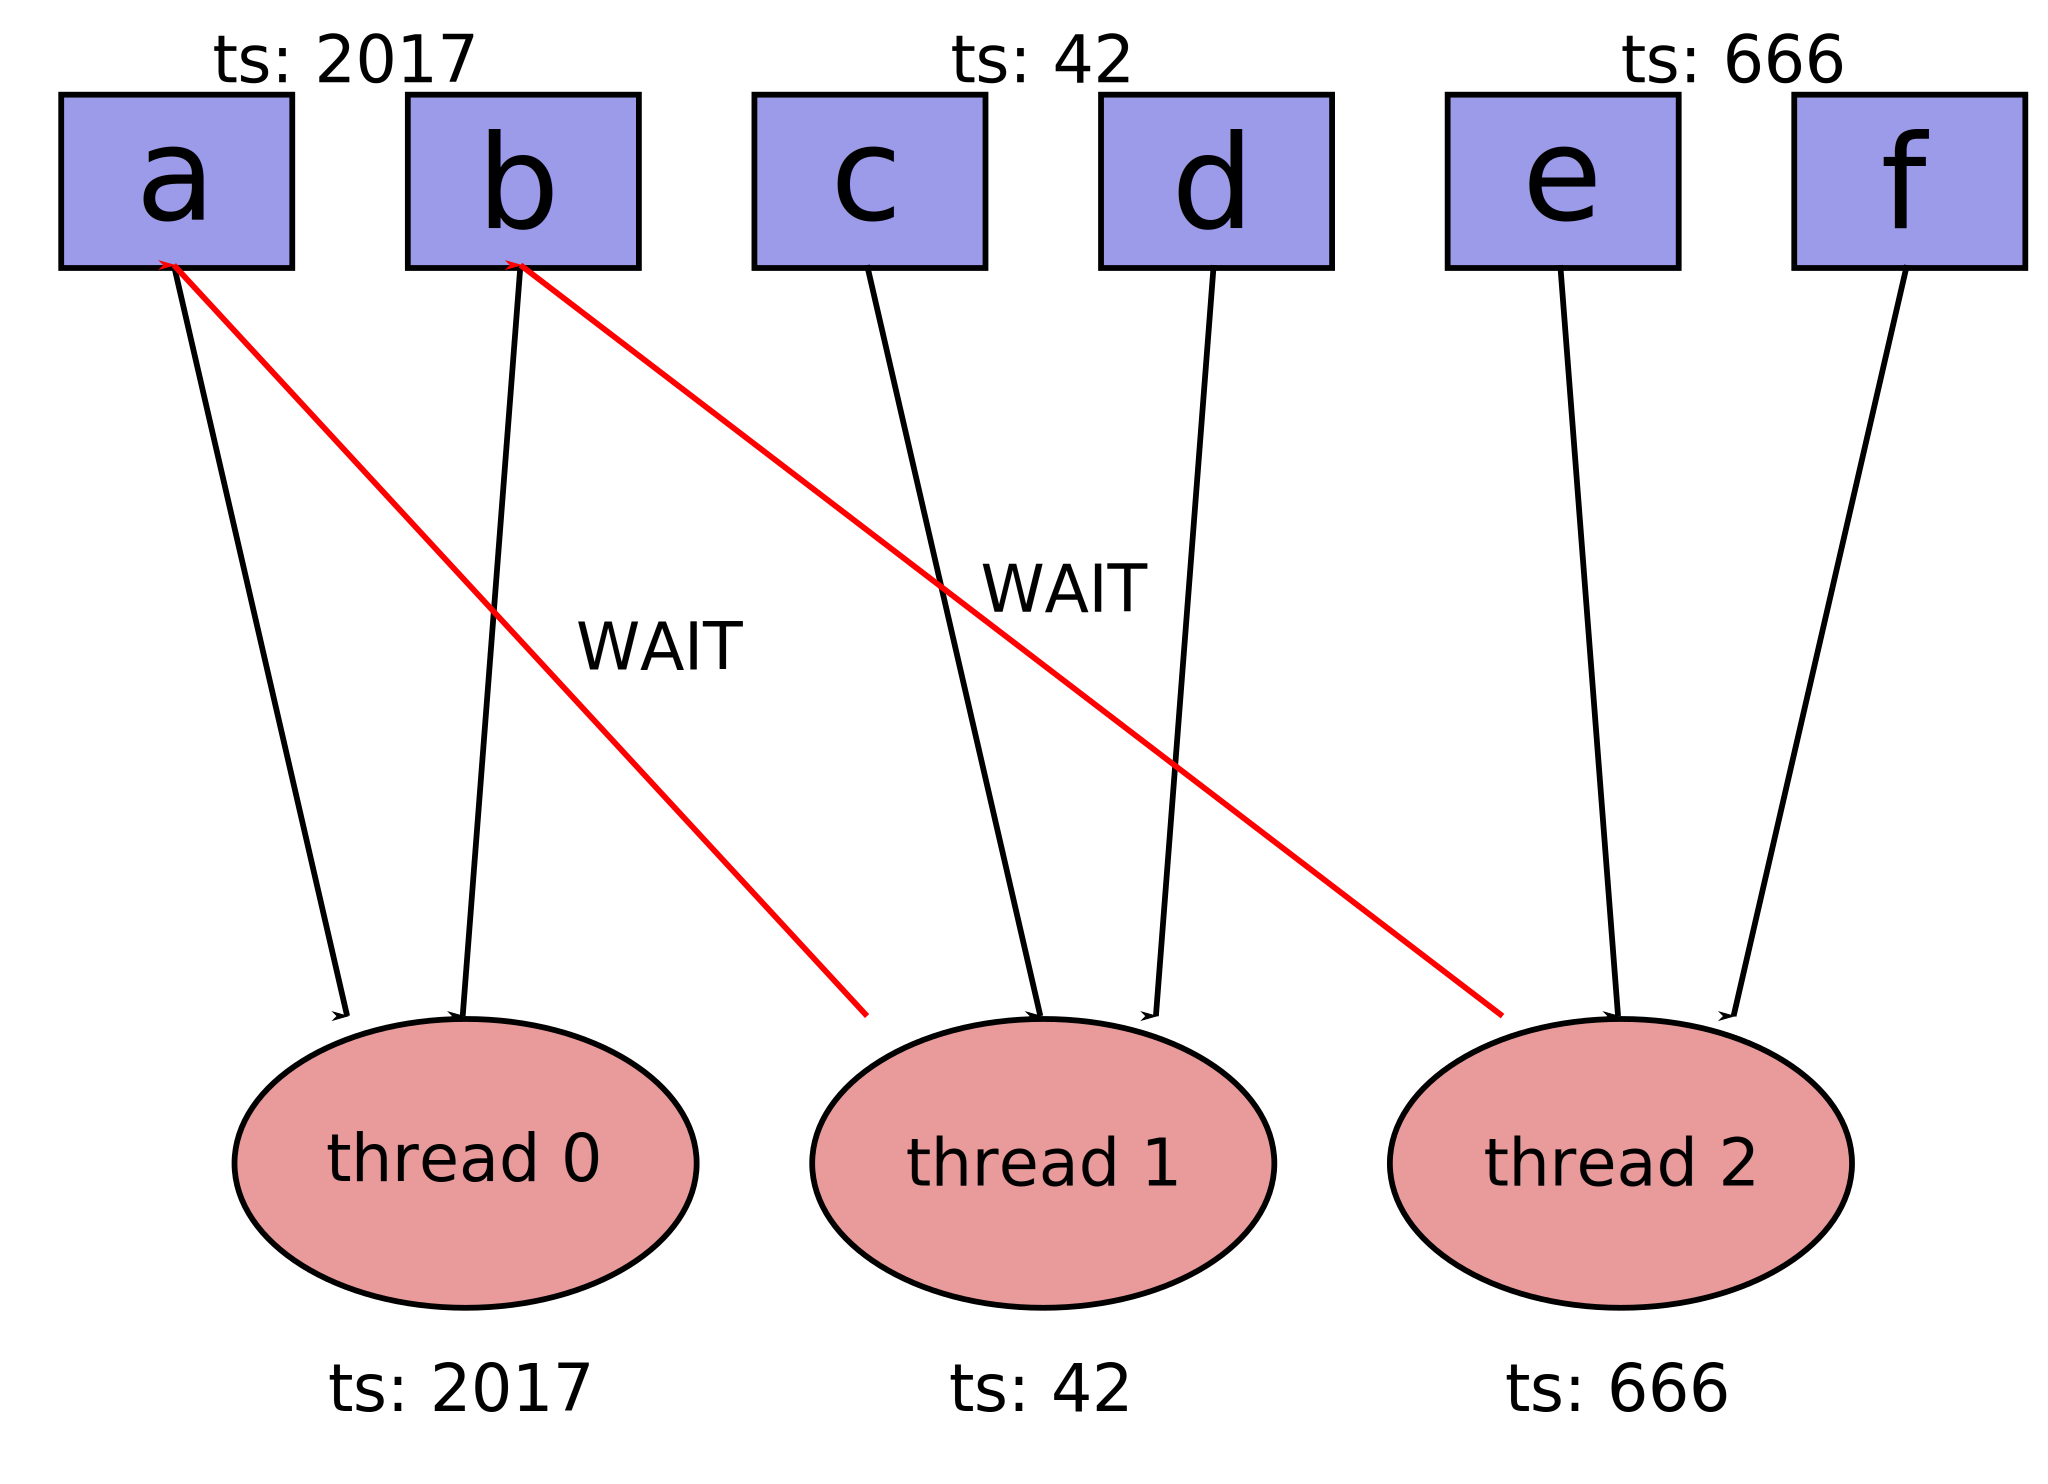
\includegraphics[height=.4\textheight]{waitdie}
\end{frame}


\end{document}
